% This is samplepaper.tex, a sample chapter demonstrating the
% LLNCS macro package for Springer Computer Science proceedings;
% Version 2.21 of 2022/01/12
%
\RequirePackage{amsmath}
% \documentclass[runningheads]{llncs}
\documentclass{llncs}
%
\usepackage[T1]{fontenc}
% T1 fonts will be used to generate the final print and online PDFs,
% so please use T1 fonts in your manuscript whenever possible.
% Other font encondings may result in incorrect characters.
%
\usepackage[T1]{fontenc}       % default encoding for Latin text
\usepackage[utf8]{inputenc}    % UTF-8 input
\usepackage{newunicodechar}    % better unicode handling
\usepackage[vietnamese,english]{babel}
\usepackage[T5]{fontenc}       % Vietnamese encoding


\usepackage{graphicx}
\usepackage[caption=false]{subfig}
% Used for displaying a sample figure. If possible, figure files should
% be included in EPS format.

\usepackage[linesnumbered,ruled,vlined]{algorithm2e}
\usepackage{hyperref}

\usepackage[backend=biber, style=lncs]{biblatex}
\addbibresource{references.bib}

\usepackage{amsmath, amsfonts, amssymb}

\usepackage{multirow}
\usepackage{makecell}
\usepackage{booktabs}

\usepackage{float}
\usepackage{siunitx}
\usepackage{csquotes}
\usepackage{enumitem}
\usepackage{bbding}

%
% If you use the hyperref package, please uncomment the following two lines
% to display URLs in blue roman font according to Springer's eBook style:
%\usepackage{color}
%\renewcommand\UrlFont{\color{blue}\rmfamily}
%\urlstyle{rm}
%
\begin{document}
%
\title{Knowledge-Enhanced \\ Vietnamese Paraphrase Identification}
%
\titlerunning{Knowledge-enhanced Vietnamese Paraphrase Identification}
% If the paper title is too long for the running head, you can set
% an abbreviated paper title here
%
%
\author{
    % Lu Xuan Minh\inst{1,2} \and
    % Nguyen Hong Minh\inst{1,2} \and
    % Nguyen Xuan Loc\inst{1,2} \and Do Thanh Thai\inst{1,2} \and Bui Tien Duc\inst{1,2} \and Quang Tran Minh\Envelope\inst{1,2}\orcidID{0000-0003-1408-2919}
}
%
\authorrunning{Lu et al.}
% First names are abbreviated in the running head.
% If there are more than two authors, 'et al.' is used.
%
%
\institute{
    % Faculty of Computer Science and Engineering, Ho Chi Minh City University of Technology (HCMUT), 268 Ly Thuong Kiet, District 10, Ho Chi Minh City, Vietnam \and Vietnam National University Ho Chi Minh City (VNU-HCM), Linh Trung Ward, Thu Duc District, Ho Chi Minh City, Vietnam \\
    % \email{\{minh.luxuanhcmut, minh.nguyenhongk22, 
    % loc.nguyen28042004, dtthai.sdh242\}@hcmut.edu.vn, tienducut@gmail.com, quangtran@hcmut.edu.vn}
}
%
%
\maketitle              % typeset the header of the contribution

\begin{abstract}

Paraphrase Identification (PI) is a fundamental task in natural language processing (NLP) that determines whether a pair of sentences convey the same meaning. This task plays a crucial role in various applications such as machine translation, computer-assisted translation, and question answering. While extensive research has been conducted in English and several other languages, Vietnamese PI remains relatively underexplored. Pre-trained language models (PLMs) have become the standard approach for tackling language understanding tasks, including PI. However, despite their rapid advancement, these models are still limited in their capacity to capture external knowledge. In this study, we propose a novel architecture that integrates pretrained language models with external knowledge for Vietnamese PI. Experimental results show that our approach, using mBERT as a base model, achieved an F1-score of 95.59\% on a combined corpus consisting of vnPara and an additional 1498 sentence pairs enriched with diverse entities. This demonstrates the effectiveness of our model in distinguishing between different entities.

\keywords{paraphrase identification \and Vietnamese \and pre-trained model \and external knowledge \and Wikipedia2Vec}

\end{abstract}
%
%
%
\section{Introduction}
Understanding whether two sentences convey the same meaning is a fundamental task in natural language understanding. PI, a task that determines whether two text fragments express the same idea, is crucial for downstream tasks, including question answering, text retrieval, text summarization, and semantic search.

In low-resource languages such as Vietnamese, accurately determining paraphrases is still a challenge due to the variety in lexical and data limitations. The terms often vary in lexical and structural features, making them challenging to identify just on the basis of surface-level semantic cues. Furthermore, detecting paraphrases from textual entailment or contradiction requires a deep semantic understanding. Recent advances in the Vietnamese PI task \parencite{dinh2021, phan2022} often leverage robust pretrained models, such as BERT \parencite{devlin2019bert} and its variants. Despite their success, these models often struggle with understanding the distinction between different named entities, reflecting the limitation of external knowledge.

In addition, Vietnamese is an \textit{analytic, non-inflectional} language in which grammatical 
relations are conveyed primarily through word order and function words rather than morphology. 
For example, the sentence ``Tôi ăn cơm'' (I eat rice) differs from ``Cơm ăn tôi'' (Rice eats me) 
only by word order, since words do not inflect for case. Orthographically, words are written as 
sequences of syllables separated by spaces, making \textit{word segmentation} a non-trivial 
preprocessing step; for instance, the single word ``học sinh'' (student) is written as two syllables 
``học'' and ``sinh''. Furthermore, Vietnamese is a \textit{tonal language} with six tones, where tone 
and context crucially determine meaning: ``ma'', ``má'', and ``mà'' are distinct words depending on tone. 
These linguistic properties, combined with frequent synonymy and flexible patterns of expression, 
pose distinctive challenges for paraphrase identification.



In this study, we propose a PI model that enhances a pretrained language model with external knowledge integration. Specifically, we incorporate named entity information from Wikipedia by training Wikipedia2Vec \parencite{yamada2020wikipedia2vec} on the latest Vietnamese Wikipedia dump to obtain entity embeddings. Our model is trained and evaluated on the vnPara corpus and an additional 1200 sentence pairs enriched with diverse entities. The experimental results indicate that our model outperforms the strong baseline, which includes BERT and its variants.

The rest of this paper is organized as follows. Section~\ref{sec:related} reviews related works. 
Section~\ref{sec:corpora} describes the corpora used in our study. 
Section~\ref{sec:methodology} presents our proposed methodology. 
Section~\ref{sec:experiment} reports the experimental setup, results, and discussion. 
Finally, Section~\ref{sec:conclusion} concludes the paper and outlines future directions.

\section{Related Works}
\label{sec:related}

%
% TRANSFORMER-BASED APPROACHES
%
Transformer's architectural breakthrough led to the emergence of BERT \parencite{devlin2019bert} and its variants such as ALBERT \parencite{lan2020albert}, ELECTRA \parencite{clark2020electra}\dots Soon, they became the state-of-the-art methods for PI. From there, the trend is to augment BERT or other similar architectures with additional structures to produce better results. One of those works is of \textcite{arase2021} where they introduced a transfer fine-tuning method that incorporates phrasal paraphrases into BERT. \textcite{xu2020} proposed the Lexical, Syntactic, and Sentential Encodings (LSSE) framework for the PI, fusing BERT-based representations with information from dependency parses. \textcite{yu2024} proposed a multi-granularity fusion model (WSTM) based on WoBERT (a word-based Chinese BERT model) that captures semantic representations at the Chinese character, word, and sentence levels with soft-attention alignment. Recently, \textcite{shi2024} formally established a connection between PI and natural language inference (NLI) with the novel framework PI2NLI.

%
% KNOWLEDGE INTEGRATION APPROACHES
%
In parallel, researchers also considered the knowledge problem in PI. There are embedding models with knowledge integration in mind such as Wikipedia2Vec \parencite{yamada2020wikipedia2vec}, E-BERT \parencite{poerner2020ebert}, etc. Our method of PI with knowledge is primarily inspired by Knowing, a model proposed by \textcite{wang2021}. Knowing enriches BERT-like models with Wikipedia knowledge by retrieving relevant outlines with BM25 \parencite{robertson2009} and making predictions based on attention and gated mechanisms.

%
% VIETNAMESE APPROACHES
%
Unfortunately, all research above is only well-experimented on English, Chinese, or other languages except Vietnamese. As far as we studied, \textcite{bach2015} was the first to plunge into the Vietnamese PI. Their method utilized string similarity measures, as they used 9 of them together with 7 representations of different abstraction levels of two input sentences. Using strong machine learning methods, they trained a model based on formed features. In the end, the highest result was obtained from the SVM classifier. \textcite{bach2015} also constructed vnPara, the first Vietnamese paraphrase corpus containing 3000 sentence pairs, which they used to evaluate on. The following work is done by \textcite{nguyen2018}. They presented a method using matching duplicate phrases and similar words. First, words in each sentence are separated using a Vietnamese WordNet \parencite{miller1995wordnet}. After removal of stop words, they proposed SimVN similarity to match words. Then, SimMat metric is calculated for prediction. They also contributed a more diverse but unbalanced Vietnamese News Paraphrase Corpus (VNPC) with 3134 sentence pairs. As \textcite{dinh2021} pointed out, these methods still relied heavily on the string-based approach. So they developed a hybrid Siamese architecture combining PhoBERT \parencite{nguyen2020phobert}, with WordNet and POS information. This hybrid method achieved strong performance, outperforming all previous models. Another usage of BERT can be seen in the work of \textcite{phan2022}, where they developed a Vietnamese Sentence BERT model for sentence embeddings, using PhoBERT as their main transformer for token embeddings. They then fine-tuned a Siamese Sentence-BERT architecture and tested it on vnPara.

%
% GAPS & OUR WORK
%
Each of these attempts has contributed greatly to improving the performance on the Vietnamese PI task. However, as far as we know, none of them have explicitly integrated external knowledge into the process. In contrast, our work, inspired by Knowing \parencite{wang2021}, will systematically fuse external knowledge into the PI model, enabling the model to reason over richer semantic meanings.


\section{Corpora}
\label{sec:corpora}

This section describes the corpora used in our experiments. We also present 
some investigations on their characteristics.


\subsection{vnPara}

This is a corpus designed specifically for the Vietnamese PI task. \textcite{bach2015} have worked to annotate the corpus, resulting in $3000$ sentence pairs with nearly balanced labels. As pointed out by \textcite{dinh2021}, main source of vnPara came from various texts collected from news websites such as news dantri.com.vn, vnexpress.net, and thanhnien.com.vn\dots


\subsection{Augmented vnPara}

This is an augmented version of vnPara. We annotated about 1500 new sentence pairs, which were chosen for their enriched named entity mentions. The main motive of such a movement is the lack of named entities in the vnPara corpus, which prevented our exploration of model performance. We ensured the corpus is labeled evenly with votes from $2$ annotators. The source to construct the augmentation is Vietnamese Wikipedia, which contains a great amount of entities.


\subsection{Some statistics on the corpora}

For further clarification, vnPara consists of exactly $3083$ sentence pairs, $1577$ of which are paraphrase pairs, the other $1506$ are non-paraphrase pairs. The augmented part we created contains evenly $749$ paraphrase pairs and $749$ non-paraphrase pairs. To monitor the improvement over named entities in the corpora, we counted entities and calculated the average number of entities per sentence (e.p.s.) as in Table~\ref{tab:count-entities}.
\begin{table}[H]
\centering
\caption{Entity count on each corpus}
\label{tab:count-entities}
\begin{tabular}{lccc}
\toprule
\textbf{Corpus} & \textbf{Total sentences} & \textbf{Total entities} & \textbf{e.p.s.} \\ \midrule
vnPara & 6166 & 6075 & 0.9852 \\
Additional data & 2996 & 7524 & 2.5113 \\
Augmented vnPara & 9162 & 13599 & 1.4843 \\
\bottomrule
\end{tabular}
\end{table}

\textcite{dinh2021} also noticed some important special cases: non-trivial paraphrase, and non-trivial non-paraphrase. The chosen measure for triviality is the Jaccard index, which indicates how much overlapping characters are from two sentences (overlap rate). Inspired by this piece, we conducted an investigation on vnPara and our augmented corpus (see Fig.~\ref{fig:jaccard}).

\begin{figure}[H]
    \centering
    \subfloat[Distribution of overlap rate in vnPara corpus\label{fig:vnpara-jaccard}]{%
      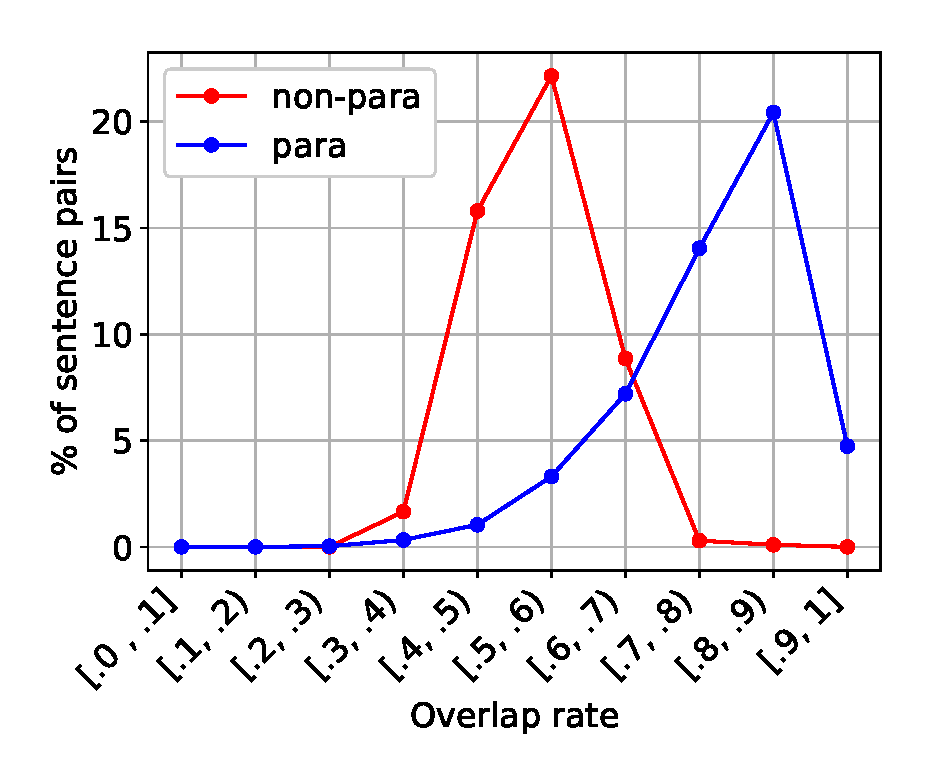
\includegraphics[width=0.32\textwidth]{images/vnpara-jaccard.eps}%
    }\hfill
    \subfloat[Distribution of overlap rate in additional corpus\label{fig:augment-jaccard}]{%
      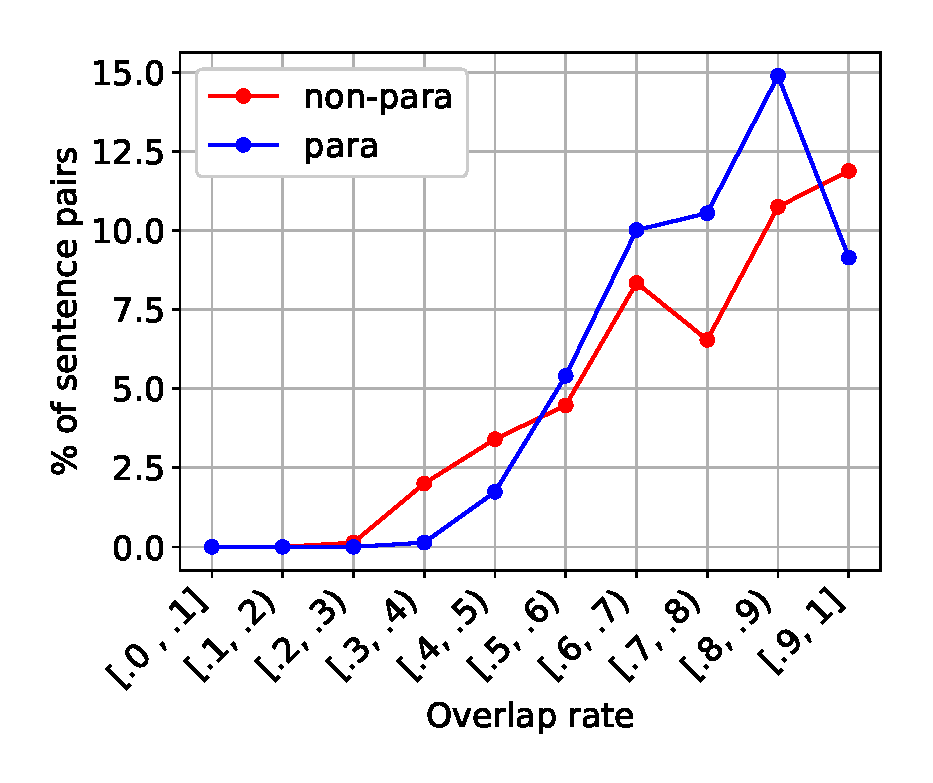
\includegraphics[width=0.32\textwidth]{images/augment-jaccard.eps}%
    } \hfill
    \subfloat[Distribution of overlap rate in augmented corpus\label{fig:augmented-jaccard}]{%
      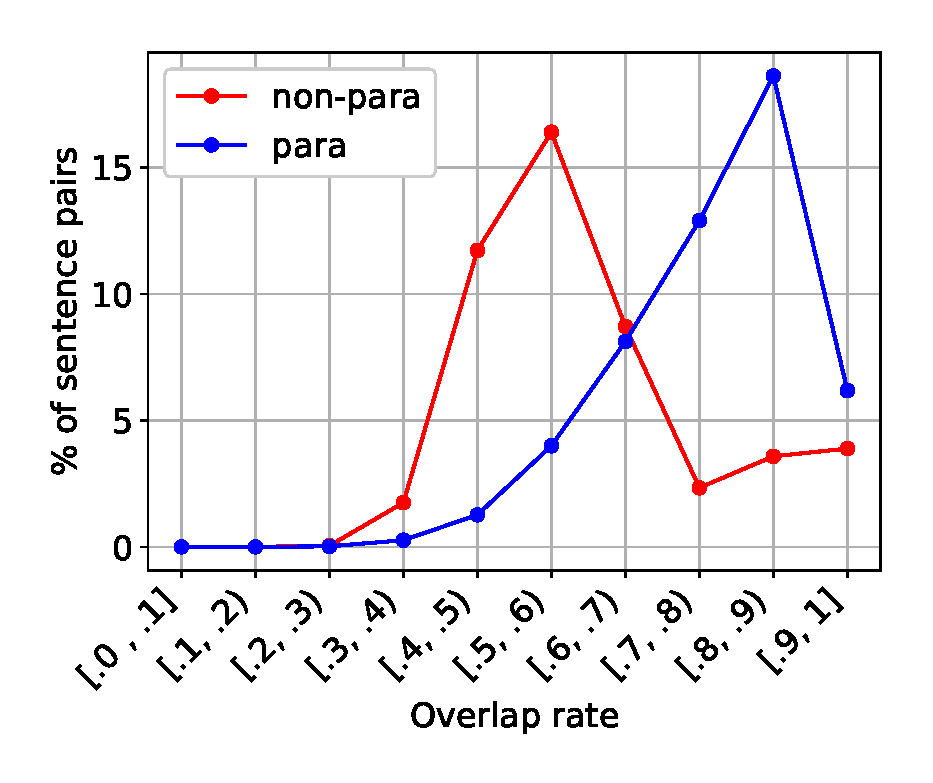
\includegraphics[width=0.32\textwidth]{images/augmented-jaccard.eps}%
    }
    \caption{Distribution of sentences across overlap rate. The x-axis is the overlap rate measured by Jaccard index divided into 10 intervals. The y-axis is the percentage of sentence pairs that is non-paraphrase (in red) or paraphrase (in blue).}
    \label{fig:jaccard}
\end{figure}

Fig.~\ref{fig:vnpara-jaccard} shows that the vnPara corpus consists of many trivial paraphrases, and non-paraphrases are distributed around the center (40\% - 70\% overlap rate) indicating that there are few non-trivial paraphrases. Our augmentation will try to balance the amount of trivial cases in the corpus. In Fig.~\ref{fig:augment-jaccard}, although our augmentation has many non-trivial non-paraphrases, collecting non-trivial paraphrases is still a great challenge as we get a high percentage of trivial paraphrases. This results in a slight shift to the right in non-paraphrase distribution, but also a spiking number of paraphrases at the high overlap rate in Fig.~\ref{fig:augmented-jaccard}.


\section{Methodology}
\label{sec:methodology}

This section describes our proposed method. For clarification, we define our notation here. Given a sentence pair $(S^1_i, S^2_i) \in \mathcal{X}$ and an external knowledge base $\mathcal{B}$, our goal is to learn a function $F(S^1_i, S^2_i, \mathcal{B}) \rightarrow \{0, 1\}$ to determine whether two sentences $S^1_i$ and $S^2_i$ have the same or different meaning, where $\mathcal{X} = \{ (S^1_1, S^2_1), (S^1_2, S^2_2), \dotsc, (S^1_n, S^2_n) \}$ denotes the training dataset, and the corresponding labels are $\mathcal{Y} = \{ y_1, y_2, \dotsc, y_n \}$. We adopted a common label convention: $0$ means that $S^1_i$ and $S^2_i$ are not paraphrases, and $1$ means otherwise.

\subsection{Overview}

To integrate external knowledge into BERT-like models, we proposed a PI model consisting of 6 key modules: BERT-like PLM, Entity Extractor, Wikipedia2Vec, Entity Attention Encoder, Entity Interaction Encoder, and Classifier (see Fig.~\ref{fig:WikiPhoBERT}).

\begin{figure}[H]
    \centering
    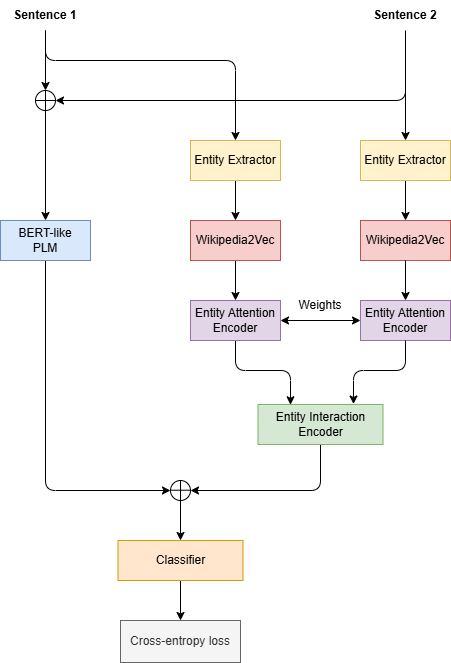
\includegraphics[width=0.5\linewidth, height=0.4\textheight]{images/WikiPhoBERT.png}
    \caption{Schema of the proposed knowledge-enhanced model. The schema highlights the interplay between 6 key modules: BERT-like PLM, Entity Extractor, Wikipedia2Vec, Entity Attention Encoder, Entity Interaction Encoder, and Classifier.}
    \label{fig:WikiPhoBERT}
\end{figure}

The base prediction module employs a PLM to encode sentence pairs. However, this base predictor overlooks the contribution of external knowledge. To address this limitation, we introduce the Entity Extractor, which identifies entities from each sentence. These extracted entities are then individually embedded using Wikipedia2Vec. The Entity Attention Encoder aggregates the entity embeddings of each sentence, assigning attention weights to the entities to learn the importance between them. The Entity Interaction Encoder simulates the semantic relationships between entities across the two sentences. Finally, the representations from the BERT-like PLM and the Entity Interaction Encoder are concatenated and passed through the Classifier for final prediction.

\subsection{BERT-like Model}

BERT-like models such as PhoBERT \parencite{nguyen2020phobert} are PLMs designed to capture contextual semantic information. Given two sentences, their combined embedding is computed as follows:
\begin{equation}
    \mathbf{e}_S = \mathrm{BERT}(S)
\end{equation}
where $S = S^1_i \oplus S^2_i$ denotes the concatenation of the two sentences. This embedding $\mathbf{e}_S$ captures the contextual information of the sentence pair.

\subsection{Entity Extractor}
We employ the \texttt{ner-vietnamese-electra-base} model developed by NlpHUST based on vELECTRA \parencite{the2020} to extract named entities from input sentences. The set of entities extracted from sentence $S^1_i$ and $S^2_i$ is denoted as:
\begin{align}
    \mathcal{E}^1_i &= \mathrm{NER}(S^1_i) \\
    \mathcal{E}^2_i &= \mathrm{NER}(S^2_i)
\end{align}

Since the extracted entities will be embedded using Wikipedia2Vec in the subsequent module, we filter out entities that do not appear in the set of Wikipedia entities, denoted by $\mathcal{E}_{\text{wiki}}$.  
The filtered entity sets are defined as follows:
\begin{align}
    \tilde{\mathcal{E}}^1_i &= \{ e \in \mathcal{E}^1_i \mid e \in \mathcal{E}_{\text{wiki}} \} \\
    \tilde{\mathcal{E}}^2_i &= \{ e \in \mathcal{E}^2_i \mid e \in \mathcal{E}_{\text{wiki}} \}
\end{align}

\subsection{Wikipedia2Vec}
Wikipedia2Vec \parencite{yamada2020wikipedia2vec} is a toolkit that jointly learns vector representations of words and entities from Wikipedia, allowing them to reside in a shared continuous vector space. This enables semantic similarity computations across both lexical and encyclopedic concepts.

Given entity $e^1_j \in \tilde{\mathcal{E}}^1_i$ and $e^2_j \in \tilde{\mathcal{E}}^2_i$, their corresponding embeddings are:
\begin{align}
    \mathbf{e}^1_j &= \mathrm{Wikipedia2Vec}(e^1_j) \in \mathbb{R}^{1 \times d} \\
    \mathbf{e}^2_j &= \mathrm{Wikipedia2Vec}(e^2_j) \in \mathbb{R}^{1 \times d}
\end{align}
where $d$ is the embedding dimension in Wikipedia2Vec space.

All $m$ embeddings $\mathbf{e}^1_j$ are stacked along the first dimension to form a matrix $\mathbf{E}_1 \in \mathbb{R}^{m \times d}$. Similarly, all $n$ embeddings $\mathbf{e}^2_j$ are stacked into $\mathbf{E}_2 \in \mathbb{R}^{n \times d}$.

\subsection{Entity Attention Encoder}
The Entity Attention Encoder aggregates entity embeddings for each sentence by assigning higher attention weights to more informative entities. To compute the importance of each entity embedding, we employed a reduced form of additive attention introduced by \textcite{bahdanau2016} as follows:
\begin{align}
    \boldsymbol{\alpha}_1 &= \mathrm{softmax} \left( \mathbf{v}^\top \tanh(\mathbf{W}_1 \mathbf{E}_1^\top) \right) \in \mathbb{R}^{1 \times m} \\
    \boldsymbol{\alpha}_2 &= \mathrm{softmax} \left( \mathbf{v}^\top \tanh(\mathbf{W}_1 \mathbf{E}_2^\top) \right) \in \mathbb{R}^{1 \times n}
\end{align}
where $\mathbf{W}_1 \in \mathbb{R}^{d_a \times d}$ and $\mathbf{v} \in \mathbb{R}^{d_a}$ are learnable parameters, $d_a$ is the hidden dimension for attention calculation.

The aggregated embeddings $\mathbf{e}_1$ and $\mathbf{e}_2$ for two sentences are obtained via weighted sums:
\begin{align}
    \mathbf{e}_1 &= \boldsymbol{\alpha}_1 \mathbf{E}_1 \in \mathbb{R}^{1 \times d} \\
    \mathbf{e}_2 &= \boldsymbol{\alpha}_2 \mathbf{E}_2 \in \mathbb{R}^{1 \times d}
\end{align}

\subsection{Entity Interaction Encoder}
The Entity Interaction Encoder is designed to capture semantic interactions between the entity representations of the two input sentences. It explicitly models both similarities and differences by combining multiple element-wise operations.

We can model the interaction between these embeddings with a simple concatenation operation proposed by \textcite{chen2017} between $\mathbf{e}_1$ and $\mathbf{e}_2$ from the previous step. In particular, we construct a joint interaction vector as follows:
\begin{equation}
    \mathbf{s} = \mathbf{W} \left[ 
    \mathbf{e}_1 \oplus
    \mathbf{e}_2 \oplus 
    \left| \mathbf{e}_1 - \mathbf{e}_2 \right| \oplus 
    \mathbf{e}_1 \odot \mathbf{e}_2 
\right]^\top \in \mathbb{R}^{d^\prime}
\end{equation}
where $\oplus$ denotes vector concatenation, $|\cdot|$ is the element-wise absolute difference, $\odot$ denotes element-wise multiplication, and $\mathbf{W} \in \mathbb{R}^{d^\prime \times 4d}$ is a learnable weight matrix that projects the concatenated vector into a shared semantic space of dimension $d^\prime$.

\subsection{Classifier}
The Classifier is a multi-layer perceptron (MLP) which is responsible for producing the final output that is ready to be converted into probabilities. It takes as input the concatenation of the sentence-pair embedding vector $\mathbf{e}_S$ and the aggregated entity interaction vector $\mathbf{s}$:
\begin{equation}
o = \mathrm{Classifier}({\mathbf{e}_S \oplus \mathbf{s}})
\end{equation}


\section{Experiment}
\label{sec:experiment}

\subsection{Experiment Setup}

\subsubsection{Evaluation Mehthod.} We'll substitute multiple PLMs such as PhoBERT \parencite{nguyen2020phobert}, mBERT \parencite{devlin2019bert}, XML-R \parencite{conneau2020xmlr}, and ViDeBERTa \parencite{tran2023videberta} in place of the embedding model. The evaluation is conducted with metrics such as accuracy and F1-score. The system will be trained on our augmented vnPara, whose splits are as follows:
    \begin{itemize}
        \item Training set: 3263 sentence pairs.
        \item Validation set: 409 sentence pairs.
        \item Testing set: 909 sentence pairs.
    \end{itemize}

\subsubsection{Configurations of Optimizer.} Our proposed model will be trained with AdamW \parencite{loshchilov2019} optimizer. We'll try different combinations of hyper-parameters. They are restricted to certain range of values as follows:
    \begin{itemize}
        \item Learning rate: [\num{1e-5}, \num{2e-5}, \num{3e-5}, \num{4e-5}, \num{5e-5}]
        \item Weight decay: [0.01, 0.02, 0.05, 0.1]
        \item Batch size: [8, 16, 32]
        \item Epochs: [2, 3, 4, 5, 6, 7, 8, 9, 10]
    \end{itemize}
    
    For more control, we employed early stopping with patience set to $3$ and minimum change of $0.01$. The loss here is the standard cross-entropy.
    
\subsubsection{Configurations of MLP.} We used the same MLP across all models. A 4-layer feed-forward network with decreasing dimensions from 2048, 1024, 256 to 2 with ReLU activations and normalizations in between each layer is utilized.

\subsection{Experimental Results}
In this section, we'll present experimental results of PI using different baseline PLMs. The most effective set of hyper-parameters for each tested model can be seen in Table~\ref{tab:hp-summary} below.
\begin{table}[H]
\centering
\caption{Effective hyper-parameters per model}
\label{tab:hp-summary}
\begin{tabular}{lcccc}
\toprule
\textbf{Model} & \textbf{Learning rate} & \textbf{Weight decay} & \textbf{Batch size} & \textbf{Epochs} \\
\midrule
\textbf{Baseline} \\
PhoBERT-base & \num{4e-5} & 0.02 & 32 & 6 \\
ViDeBERTa-xsmall & \num{3e-5} & 0.02 & 32 & 8 \\
ViDeBERTa-base & \num{5e-5} & 0.05 & 8 & 8 \\
mBERT & \num{5e-5} & 0.01 & 32 & 6 \\
XLM‑R & \num{5e-5} & 0.02 & 32 & 6 \\
\midrule
\textbf{Ours with} \\
PhoBERT-base & \num{2e-5} & 0.01 & 16 & 6 \\
ViDeBERTa-xsmall & \num{2e-5} & 0.05 & 8 & 10 \\
ViDeBERTa-base & \num{2e-5} & 0.01 & 8 & 6 \\
mBERT & \num{2e-5} & 0.01 & 16 & 10 \\
XLM‑R & \num{2e-5} & 0.1 & 16 & 8 \\
\bottomrule
\end{tabular}

\end{table}

Table~\ref{tab:test-summary} demonstrates the testing results such as accuracy, precision, recall, and F1-score obtained from evaluating trained models on the testing set. The highest value is highlighted in boldface.
\begin{table}[H]
\centering
\caption{Summarized evaluation results with different baselines}
\label{tab:test-summary}
\begin{tabular}{lcccc}
\toprule
\textbf{Model} & \textbf{Accuracy} & \textbf{Precision} & \textbf{Recall} & \textbf{F1-score} \\
\midrule
\textbf{Baseline} \\
PhoBERT-base & 0.7844 & 0.7905 & 0.7844 & 0.7840 \\
ViDeBERTa-xsmall & 0.6744 & 0.7032 & 0.6744 & 0.6814 \\
ViDeBERTa-base & 0.7140 & 0.7136 & 0.7140 & 0.7137 \\
mBERT & 0.7316 & 0.7415 & 0.7316 & 0.7314 \\
XLM‑R & 0.6733 & 0.8036 & 0.6733 & 0.6895 \\
\midrule
\textbf{Ours with} \\
PhoBERT-base & 0.9197 & 0.9205 & 0.9197 & 0.9198 \\
ViDeBERTa-xsmall & 0.9032 & 0.9071 & 0.9032 & 0.9030 \\
ViDeBERTa-base & 0.9285 & 0.9285 & 0.9285 & 0.9285 \\
mBERT & \textbf{0.9560} & \textbf{0.9572} & \textbf{0.9560} & \textbf{0.9559} \\
XLM‑R & 0.9461 & 0.9462 & 0.9461 & 0.9461 \\
\bottomrule
\end{tabular}
\end{table}


\subsection{Discussion}

%
% ABSTRACT POINT
%
Evidenced by Table~\ref{tab:test-summary}, our proposed method unequivocally achieved significant enhancements for the baseline PLMs. Improvements are yielded across all metrics compared to their respective baselines.

%
% INTERPRETING RESULTS
%
However, the amount of enhancements is different for different architectures. Let's discuss monolingual models (PhoBERT and ViDeBERTa) first. When integrating with PhoBERT-base, we got a relatively high F1-score of 91.98\%, a substantial gain of 13.58\% from 78.40\% at baseline. We observed even stronger improvements with ViDeBERTa as ViDeBERTa-xsmall achieved 90.30\% (22.16\% gain) and ViDeBERTa-base achieved 92.85\% (21.48\% gain) in F1-score. Notably, the highest improvement came from multilingual models (mBERT and XLM-R). Our model with XLM-R gained the most with 94.61\% in F1-score (improved by 25.66\%). But the highest results belonged to mBERT, which reached 95.59\% in F1-score (22.45\% gain). We observed that our approach yields better performance for multilingual models than monolingual models.


%
% LIMITATIONS
%
Despite good results, there are still persistent limitations with our method. The entity representations did not strongly expand their contexts into the whole sentence. The only occurrence of the interaction between entities and sentences lies in the feed-forward network near the output layer of our model. It wasted the positional information of the entities and the contexts around them.

For detecting entities, a NER-specific PLM was employed. The accuracy of finding entities relies heavily on the accuracy of the NER model. Even if the NER model was decent at its job, the Wikipedia2Vec model could still cause problems. In detail, all entities that are not appearing in Wikipedia2Vec space are discarded. However, Wikipedia2Vec is too sensitive to the form of the words. Rewriting a name with different forms can lead to non-existing entities.

Another notable limitation came from the corpora. We augmented vnPara with additional data, but as Fig.~\ref{fig:augment-jaccard} shows, the non-trivial paraphrases are still very limited since they cluster at the high overlap rate, producing lots of similar sentences that are paraphrases. Our final augmentation hardly shifts this fact.


\section{Conclusion}
\label{sec:conclusion}

In this paper, we have explored the knowledge problem in Vietnamese PI. We proposed a model utilizing a NER model and Wikipedia2Vec to extract knowledge through named entities. We trained Wikipedia2Vec on the latest Vietnamese Wikipedia dump for this goal. Our model aggregates the entity embeddings with an additive attention mechanism. The entities are then compared through a simple concatenate operation to produce the final prediction. In the end, we have successfully enhanced PLMs such as PhoBERT, ViDeBERTa, mBERT, and XLM-R, achieving a 13\%--26\% gain in F1-score on our augmented vnPara corpus. Most notably, our model with mBERT as a base model attained the highest F1-score of 95.59\%.

Despite its performance, our model still faces many problems that warrant further focus in the future. To reduce the dependency on the NER model, we plan to replace it with other extraction techniques such as retrieval with BM25 or vectorized databases. We also plan to solve the Wikipedia2Vec misalignment by using BERT-like models themselves to encode the knowledge. Finally, instead of only Wikipedia, we intend to incorporate other knowledge bases such as WordNet into our method in the near future.

\begin{credits}
\subsubsection{\ackname} We would like to thank Ho Chi Minh City University of Technology (HCMUT), VNU-HCM for the support of time and facilities for this study.
\end{credits}

\printbibliography

\end{document}
